\chapter{Physical properties of transition metal dichalcogenide monolayers}

\section{Crystal structure and symmetries}

\begin{figure}[t]
	\centering
	\begin{subfigure}{0.30\textwidth}
		\caption{}
		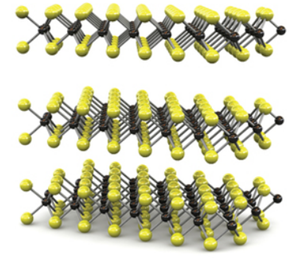
\includegraphics[height=.9\textwidth,left]{3d}
		\label{crystal1}
	\end{subfigure}
	\begin{subfigure}{0.30\textwidth}
		%\centering
		\caption{}
		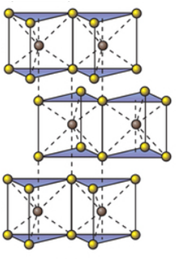
\includegraphics[height=.9\textwidth,center]{triangles}
		\label{crystal2}
	\end{subfigure}
	\begin{subfigure}{0.30\textwidth}
		\centering
		\caption{}
		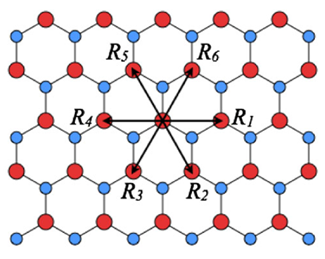
\includegraphics[height=.9\textwidth,right]{topview}
		\label{crystal3}
	\end{subfigure}
	\caption{Crystal structure of \tmds\!: \textbf{A} \tmds are composed of large sheets of transition metal atoms sandwiched in between chalcogenite atoms. The covalent bonds strongly hold the layers together in-plane, while the individual sheets are only weekly bound by van-der-Waals forces. \textbf{B} In the 2\textsc{h} phase, the unit cell of \tmds has a triagonal prismatic shape with the transition metal in the center, between two triangles of chalcogenite atoms. \textbf{C} Viewed from the top, \tmds show a hexagonal lattice structure. However, because of the structure of the unit cell, the inversion symmetry is broken. Graphics from\cite{wang_electronics_2012, xiao_coupled_2012}}\label{crystal}
\end{figure}

Like to all layered materials, \tmds consist of large covalently bound sheets, that are held together by the weak van-der-Waals force. And similar to graphite these sheets have a hexagonal lattice structure and form layers of only one unit-cell in the out-of-plane axis. It is the details of these unit-cells that distinguish \tmds from graphite and other layered materials. The fundamental building block of the bulk crystal is a single sheet -- the monolayer -- that consists of three atomic layers -- A layer of transition metal atoms like tungsten (\textsc{w}) or molybdenum (\textsc{M}{\footnotesize o}) sandwiched between two layers of chalcogen atoms like sulfur (\textsc{s}), selenium (\textsc{s}{\footnotesize e}) or tellurium (\textsc{t}). This thesis is primarily concerned with tungsten-based \tmds\!: \wse and \ws\!. \textsc{Tmd}s can be in different phases, that have a different crystal structure as well as different electronic properties. The stable semiconducting phase is called 2\textsc{h}. In this configuration every transition-metal atom has six neighboring chalcogen atoms and forms a trigonal prismatic unit-cell, with the transition-metal in the center as depicted in figure \ref{crystal} \textbf{B}. A \tmdg monolayer exhibits a $\mathcal{D}^1_{3h}$-symmetry. The unit-cell is invariant under 3-fold rotation as well as in-plane reflection. In the top-view (see figure \ref{crystal} \textbf{C}) this looks similar to the hexagonal lattice structure of graphene, but with the key difference of a broken inversion symmetry. When the unit-cell is inverted with the transition metal atom as its inversion center, the chalcogen atoms wind up in empty locations as with any possible inversion point.

This has two important consequences, regarding the band structure. As in graphene, the reciprocal lattice is hexagonal. However at the edges of the Brilloin zone the degeneracy of the $K$-points is broken and instead of the characteristic Dirac cone of graphene, \tmdg monolayers form a direct band gap (see figure \ref{bandgap}). The latter makes these materials very efficient photonic emitters, while the former enables so-called valley polarization. The local minima/maxima of the band structure (valleys) at the $K$ and $K'$ points can be selectively addressed with circularly polarized light of opposite helicity. The corresponding emission is of the same polarization as the incident beam. This effect demonstrates control over a new degree of freedom, the ``valley index'' and opened up the field of ``valleytronics'', in which analogous to electronics and spintronics, the valley degree of freedom could be used by means of information processing\cite{wang_electronics_2012, xiao_coupled_2012}. Additionally the valence band of \tmds, that is mostly composed of the $d$-orbitals of the heavy transition metal atoms exhibits strong spin-orbit coupling. The large splitting in the order of 150 meV couples the optical transition energy to the spin of the excited electron. Because this splitting is reversed in $K'$ the valley-index is also coupled to the spin.

\section{Excitons in \tmdg monolayers}\label{theory_exciton}

What sets the light emission of \tmds apart from conventional direct band gap semiconductors is, that even at room temperature, the photoluminescence (\pl\!) is dominated by the recombination of excitons. Excitons are bound pairs of an electron and a corresponding hole. In bulk semiconductors this bound state has a very low binding energy due to dielectric screening. The 2\textsc{d}-geometry of \tmdg monolayers however effectively reduces the screening effect, which results in strong Coulomb interaction between electron and hole. This raises the exciton binding energy to approximately 500 meV, which enables excitons to form well above room temperature\cite{chernikov_exciton_2014}.
The thinness of \tmdg monolayers has additional implications. Because the electric dipole field of the exciton extends beyond the boundaries of the crystal, the dielectric environment has a big influence on the optical spectrum\cite{stier_probing_2016, borghardt_engineering_2017, jakubczyk_impact_2018}. Impurities such as microscopic water droplets or dangling bonds of silicon oxide can induce localized potentials, broadening the linewidth of the \pl features, thus complicating spectroscopic studies. On the other hand, this high sensitivity could be used in quantum sensing applications to optically probe or visualize electric or magnetic proximity effects\cite{neumann_opto-valleytronic_2017}\red{referenz}.


\begin{figure}[t]
\centering
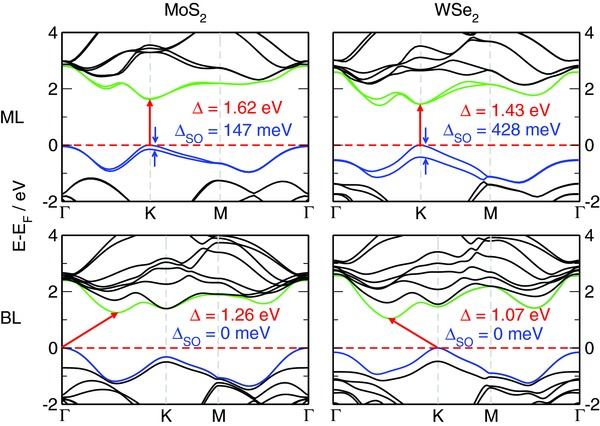
\includegraphics[width=.7\textwidth]{bandstructure}
\caption{Band structure for \mos and \wse mono- and bilayers. In the limit of a single atomic layer \tmds form a direct band gap at the $K$-point and the valence band is strongly split due to spin-orbit coupling. Graphic taken from \cite{zibouche_transition-metal_2014_2}.}
\label{bandgap}

\end{figure}

\section{Spectral composition of ws\textup{e}$_2$}\label{composition}

\begin{figure}[t]
\centering
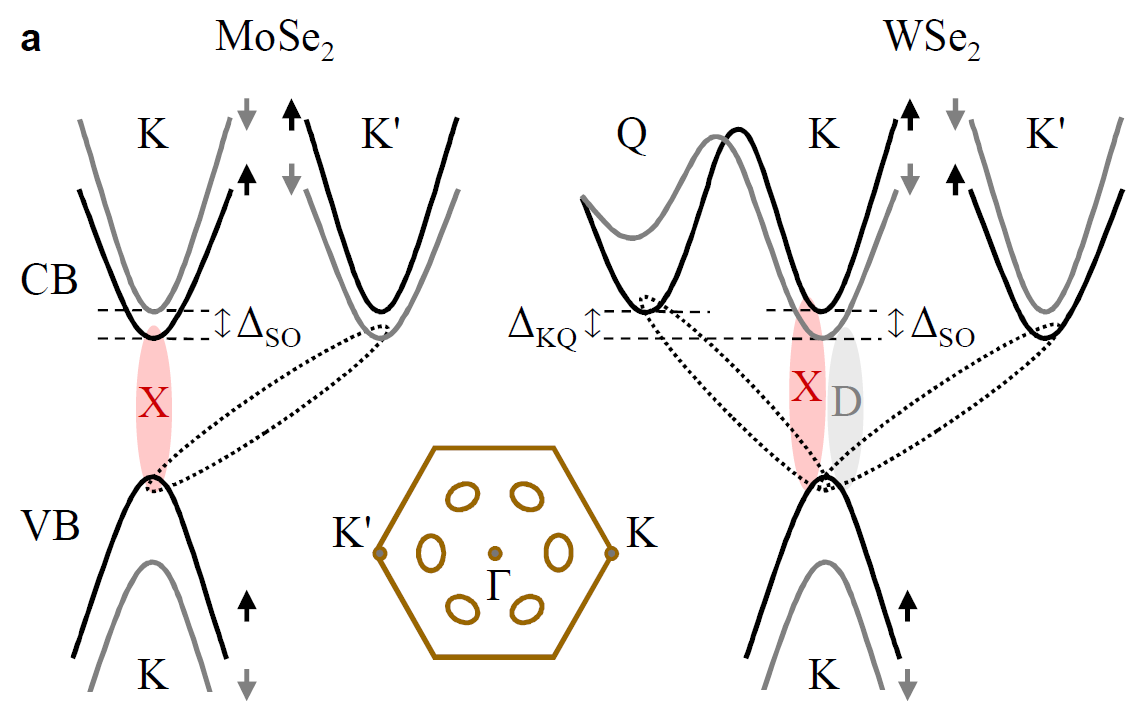
\includegraphics[width=.8\textwidth]{Band_structure_momentum_dark}
\caption{}\label{bands}
\end{figure}

The optical spectrum of \tmds both in reflection and \pl is dominated by excitonic effects. In \wse especially the \pl spectrum shows a rich ensemble of characteristic spectral features, that so far have not been identified completely and the discussion around the underlying processes is still active.

For \hbng encapsulated \wse the main exciton resonance ($X$) is located at around 1.72 eV. This resonance corresponds to the creation and annihilation of an exciton in the $K$ valley with electron and hole having a parallel spin component ($X_l$). The corresponding exciton with antiparallel spins is often called the dark state as its ``spin-forbidden'' ($D$/$X_u$). Its radiative decay is only allowed in-plane, because of symmetry reasons\texttrademark. Because of spin-orbit coupling this state lies about 40 meV lower than the bright exciton\cite{echeverry_splitting_2016}. The \pl from these excitons can be collected from the side or with a high numeric aperture objective, that catches light not directly emitted in the $z$-direction\cite{robert_fine_2017, wang_-plane_2017}. In the presence of free charges, either holes or electrons, excitons can interact with them to form trions that are associated with a redshift of 20-30 meV\cite{courtade_charged_2017}. While these properties can be predicted by modeling the trion as a three-body quasi particle, its precise nature still remains under discussion. The most contrarian interpretation to the helium-like bound state is a so-called fermi polaron. In a charged regime excitons behave like an impurity in a ``sea'' of electrons, forming the polaron quasi particle\cite{sidler_fermi_2016, efimkin_many-body_2017,schmidt_fermi_2012}.

The spectrum of \wse shows additional features, have so far escaped thorough understanding. In light of strong sample-to-sample variation, they are commonly attributed to localized effects, like defect-induced quantum dots or local doping\cite{kato_optical_2014, zhang_defect_2017}, that create trapped excitons. Improved fabrication techniques like mechanical exfoliation and the usage of \hbng as a substrate (see section \ref{exfoliation}) have enabled experimentalists to measure spectra with very little defects and narrow linewidths, that still show a rich class of features, that are reproducible in other samples as well as in the samples used in this work.

\subsection{Phonon sidebands}\label{sidebands}

Our group recently proposed a model identifying these peaks as phonon side-bands of momentum-indirect excitons\cite{lindlau_identifying_2017}. It has recently been shown, that in contrast to molybdenum-based \tmds \wse actually shows an indirect band gap\cite{zhang_probing_2015, hsu_evidence_2017}. As can be seen in figure \ref{bands}, the $Q$-valley lies energetically close to the $K$-valley and is suggested to be lower than the upper $K$-valley, that participates in the direct spin-like exciton transition. This could point to a high population of excitons composed of electrons in $Q$ as well as in the lower lying spin-like $K'$-valley. While both these states are spin-allowed, momentum conservation prevents them from radiatively decaying in a single-photon process. Instead they can recombine with assistance of an additional phonon, carrying the inter-valley momentum. For momentum conservation to hold the following equations has to be fulfilled for momentum-indirect excitons in $Q$ or $K'$ respectively:
\begin{align}
	\vec{k}_K + (\vec{k}_K - \vec{k}_{Q/K'}) &= \vec{k}_K + \vec{k}_\gamma + \vec{k}_{phonon}\\
	\Rightarrow \vec{k}_{phonon} &\mbeq \vec{k}_K - \vec{k}_{Q/K'}
\end{align}
Because of the hexagonal structure of the Brilloin zone $\vec{k}_K - \vec{k}_{K'}$ simply equals a phonon in $K$ whilst $\vec{k}_K - \vec{k}_{Q}$ is conveniently close to a phonon in $Q$. Crystal vibrations in \tmds can have three acoustic and six optical modes, but only two acoustic and three optical modes can couple to charge carriers. This leaves a total of five possible phonon sidebands for both $Q$- and $K'$-indirect excitons, neglecting processes involving more than one phonon. Corresponding, theoretically calculated energies can be found in \ref{phonons}\cite{jin_intrinsic_2014}. The phonon replica would appear as a peak redshifted by these energy values. For $K'$-indirect excitons the positions of the peaks can be inferred directly, since the energy splitting between the spin-like and spin-unlike exciton is known and both features can be measured. The $Q$-valley however has no direct decay channel. Its energy thus has to be fixed inductively, by looking for peaks that fit the pattern, given by the phonon energies and calculate backwards.

\begin{figure}[t]
\centering
\begin{tabular}{lllll}
\hline
\hline\\
Mode&K&Q\\
\hline\\
TA&15.6&11.6\\
LA&18.0&14.3\\
TO(E')&26.7&27.3\\
LO(E')&31.5&32.5\\
A$_1$&31.0&30.4\\
\\\hline


\end{tabular}
\caption{\cite{jin_intrinsic_2014}}\label{phonons}
\end{figure}
\cite{van_der_donck_excitons_2018} 

\section{The valley zeeman effect}\label{zeeman}

A splitting of spectral lines in presence of a magnetic field has been studied for over a hundred years and is called the Zeeman effect, named after the scientist first measuring it in the spectral lines of sodium. The shift of different energy levels in an atom results from the magnetic moment of the state, caused by its orbital angular momentum and spin. Solid crystals are essentially large ensembles of atoms that merge atomic orbitals to form the electronic band structure, that can shift in a magnetic field just as orbitals of single atoms. The 2\textsc{d}-nature of \tmdg monolayers and their broken degeneracy of the $K$ and $K'$ point gives rise to a meta-phenomenon called  the ``valley Zeeman effect'', that leads to a shift in the band gap energy that is different for both valleys, leading to a split of spectral lines with different circular polarization\cite{srivastava_valley_2015}. In the vicinity of the $K$ point the band structure is dominated by the large $d$-orbitals of the transition metal atoms. The hybridized $d_{x^2-y^2} \pm id_{xy}$ orbitals carry oribtal angular momentum and a magnetic dipole moment. The \tmd-geometry confines electron movement to the 2\textsc{d} plane, forcing the magnetic moment to either point upwards or downwards out of plane. This direction is exactly opposite at the $K$ and $K'$ points, shifting the valence band energy, and thus the band-gap in opposite directions. For the direct exciton transition the observed magnetic moment has a value of $\pm$2$\mu_B$, leading to a valley splitting of $\Delta_{K,K'}$=4$\mu_BB$. The prefactor in this equation is often called the $g$-factor and is given in units of the Bohr magneton $\mu_B$=$e\hbar/2m_e$.

The precise prediction of the $g$-factor for different states is a nontrivial task as predicting the shift in the band structure requires knowledge of the quasi particle effective mass and has to take into account the spin of the excitons components and its magnetic moment, that is governed by the strong coulomb exchange interaction. \cite{rybkovskiy_atomically_2017}